\section{Internet Telephony}
\label{sec:measurement:voip}


In this section, we use production data from a large VoIP service 
provide \skype to quantify the impact of network metrics on 
audio call quality, and patterns of poor network performance. 
%The observations motivate the need for and the design 
%requirements of \hybrid.

\subsection{Dataset}
\label{subsec:measurement:voip:dataset}

The dataset from \skype consists of a sampled set of $430$ 
million audio calls drawn from a seven month period. 
%\camera{They are sampled from \cmvnp{the set of} calls made by \cmvnp{clients on the} \fillme platform \cmrvnp{and they are the only calls with recorded} \cmvnp{and for which} performance metrics \cmvnp{are recorded}.}
%\vnp{I wonder if the low count is because we are only considering calls for which the performance metrics are recorded. If so, we should say so.} 
The sampled set includes both calls that use the 
\direct path (e.g., BGP-derived) between the caller 
and the callee %(\cameraremove{$40\%$}\camera{$15\%$} of the calls in the set) 
as well as calls that are relayed through managed 
relay nodes distributed across datacenters in different 
locations. % (the remaining \cameraremove{$60\%$}\camera{$85\%$} of the calls). 
%\vnp{We say "randomly sampled" and then also say "sampled set is chosen" (which appears to contradictory to "random") and furthermore give the 40-60 split (which, together with "random", leaks info on how much relaying happens). I would suggest striking off "randomly".} 
Note that today such relaying is typically employed for 
connectivity (e.g., firewall or NAT traversal) rather than 
for performance optimization (which is our focus here).
That is, the only instances of relaying in our passively 
collected dataset correspond to the caller and callee being 
unable to establish a direct connection. 
Despite this bias, the dataset offers a {\em panoramic} view 
across diverse end-points from $1,905$ ASes across $126$ 
countries. Table~\ref{tab:dataset} summarizes the statistics.
% \footnote{In general, it is unclear if reachability and performance are correlated.}


\begin{table}[t!]
\centering
\begin{small}
\begin{tabular}{cc}
\hline
{\bf Time}          & $2015.11.15 - 2016.05.30$ \\ \hline
{\bf Calls}         & $430$M                  \\ \hline
{\bf Users}         & $135$M                 \\ \hline
{\bf ASes}          & $1.9$K                  \\ \hline
{\bf Countries/regions}     & $126$                 \\ \hline
%{\bf Relay locations} & $74$ \\  \hline    
%\end{footnotesize}
\end{tabular}
\end{small}
\caption{\skype dataset summary.}
\label{tab:dataset}
\end{table}

To the best of our knowledge, our work is the first to 
study the quality of Internet telephony calls at such 
a large scale.
There are several characteristics that make this dataset
stand out: a large fraction of calls are international 
($46.6\%$), inter-AS ($80.7\%$), and wireless ($83\%$). % Specifically, \cameraremove{$87\%$}$46.6\%$ of calls in our dataset are between users in different countries, \cameraremove{$93\%$}$80.7\%$ are between users in different AS domains, and \cameraremove{$74\%$}$83\%$ have at least one client using a wireless connected device. 
These characteristics allow us to study the performance 
of Internet telephony over a much greater diversity of 
Internet paths than has been considered in prior studies,
% many more paths in the Internet compared to the prior analyses
 where traffic was mostly US-centric (e.g., 
 \cite{xbox-sigcomm09}) or confined to server-client 
 paths (e.g., \cite{sigcomm11conviva}) or academic 
 sites (e.g., PlanetLab~\cite{iplaneosdi}).
%\jc{In general, we should highlight this dataset is the best for analyzing and improving our application, rather than saying its a better dataset for analyzing network performance.}
 
 % between nodes that were close to each other (e.g., P2P~\cite{p2pXXX}), between clients and servers (e.g., video streaming~\cite{videoXXX}), or US-centric (e.g., online gaming~\cite{xbox}).
	
 % http://www.cs.yale.edu/homes/yong/publications/XY07.pdf
 
 % http://ccr.sigcomm.org/archive/2001/apr01/ccr-200104-cole.pdf

%\jc{Dropped the sparseness part here. Better not to mention it here to avoid confusing readers.}



Each call is associated with three metrics of network 
performance: $\left(i\right)$ round-trip time (RTT), 
$\left(ii\right)$ loss rate, and $\left(iii\right)$ jitter. 
(We do not analyze bandwidth given the low data rate 
typical of VoIP streams.) 
These network metrics are calculated by the \skype 
clients in accordance with the RTP 
specifications~\cite{rtp-rfc3550} and correspond to 
the average value of each metric over the entire duration 
of a call. 
(More detailed network metrics such as transient latency 
spikes or loss bursts are not reported.) 
To understand the characteristics of \direct Internet routing,
this section focuses only on default-routed (BGP-derived) 
calls.


\subsection{Call Quality \& Network Performance}
\label{subsec:measurement:voip:quality}

\begin{figure}[t!]
\centering
\subfloat[\small{PCR vs. RTT}]
{
        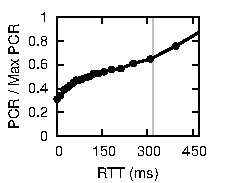
\includegraphics[width=0.3\textwidth]{figures/Via-Quality-vs-Pcr-RTT.pdf}
        \label{subfig:pcr-rtt}
}
\subfloat[\small{PCR vs. Loss}]
{
        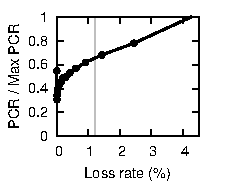
\includegraphics[width=0.3\textwidth]{figures/Via-Quality-vs-Pcr-Loss.pdf}
        \label{subfig:pcr-loss}
}
\subfloat[\small{PCR vs. Jitter}]
{
        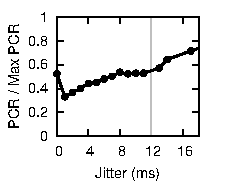
\includegraphics[width=0.3\textwidth]{figures/Via-Quality-vs-Pcr-Jitter.pdf}
        \label{subfig:pcr-jitter}
}
\caption{Network performance metrics have considerable 
impact on user experience (poor call rate or PCR); 
y-axis normalized to the maximum PCR. Vertical gray lines 
show the thresholds for poor network performance.}
\label{fig:pcr}
\end{figure}

%To quantify the call quality, we first consider an empirical approach. 
For a small random fraction of calls in \skype, users label the
call quality on a discrete $5$-point scale, ranging from $1$ 
(worst) to $5$ (best). 
%However, %PCR is subjective and to limit the imposition on users, \skype obtains user rating for only a small fraction of the calls. 
Consistent with the operational practice in \skype, we deem 
the calls with a rating of $1$ or $2$ as ``poor'', and use the 
fraction of such calls, termed as the {\em Poor Call Rate (PCR)}, 
as an empirical metric of user experience. 
Besides PCR, prior work also has provided analytical models to 
translate the network metrics into a measure of audio call quality, 
called the {\em Mean Opinion Score (MOS)} (e.g., \cite{cole}).
%% , ranging from 1 (bad) to 5 (excellent) on a continuous scale. Here we use the model given in \cite{cole}, which has also been used widely in other studies. Though MOS is objective and can be calculated from network metrics of any call, it \red{produces a single mean score for a call, which} does not capture the range of user experiences \red{that would be seen even} under \red{similar} average network conditions \red{(e.g., due to transient badness)}.

%The dataset from \skype provides visibility into the network performance metrics for a wide range of end-to-end paths traversed by calls. Prior work has translated these metrics into a measure of audio call quality, called the {\em Mean Opinion Score (MOS)}, ranging from 1 (bad) to 5 (excellent) on a continuous scale. Here we use the model by Cole and Rosenbluth~\cite{cole} that has also been used widely in other studies. 
%Separately, we also consider an empirical approach. For a small, random fraction of calls in \skype, users label the call quality on a discrete 5-point scale, ranging from 1 (worst) to 5 (best).
%% as ``good'' or ``bad''.~\footnote{The rating, in practice, is on a scale of 1 to 5. Scores of $\leq 2$ count as ``bad''.} We use the fraction of calls 
%Consistent with the operational practice in \skype, we deem the calls with a rating of 1 or 2 as ``poor'', and use the fraction of such calls, termed as the {\em Poor Call Rate (PCR)}, as the metric of user experience. 

%%%\red{Both model-based MOS and empirically-derived PCR have their advantages and limitations. The main advantage of PCR is that it directly relates to user-perceived experience; indeed, it is of prime importance in the context of \skype, based on our conversations with their engineers. Moreover, it reflects, to an extent, the {\em distribution} of user experience in that it reports the fraction of calls rated as poor instead of just a single mean score for call quality. However, being user-derived also makes it subjective. Users may be biased in whether and how they rate calls, based on extraneous factors (e.g., their mood). More importantly, computing PCR involves first polling users, an imposition that limits \skype to obtaining user rating for a small fraction of the calls. 
	
%%%On the other hand, a MOS model produces an objective score, which could be computed for all calls, since the network metrics that it depends on could, in principle, be gathered for all calls, with little overhead~\footnote{For our study, though, we only had access to network metrics for a subset of 54 million XXX out of the XXX calls in the corresponding period.}. The main limitation, though, of a MOS model is that it produces a single mean score, which would not reflect the range of user experiences under the given average network conditions. On a related note, a MOS model which only works with the average network metrics for a call (which is what is available in \skype) might not register transient badness (e.g., a loss burst), which could nevertheless negatively impact user experience.}

%%Both model-based MOS and empirically-derived PCR 
%Both PCR and MOS have their advantages and limitations. 
%%Being user-derived makes PCR subjective but it reflects, to an extent, 
%Since PCR is based on per-user feedback, it reflects the {\em distribution} of user perception under the same network performance, but it is subjective and the imposition of polling users limits \skype to obtaining user rating for only a small fraction of the calls. 
%MOS, on the other hand, is objective and can be calculated from network metrics of any call,
%%calculated from the average network metrics for a call and can be calculated for all the calls in the dataset. 
%%But since it only produces a single mean score, 
%but it does not capture the range of user experiences under the given average network conditions.

%%Here, we use an approach that combines the advantages of both.% an empirically-derived PCR (in terms of relating to the distribution of user experience) and a MOS model (in terms of being objective and easy to compute for all calls).} 
In this section, we show that both PCR and MOS are 
well-correlated with network metrics. %%, \red{though PCR is more sensitive}. 
Then, we identify suitable {\em thresholds} for poor call 
performance on the network metrics of RTT, loss and jitter. 
Since our goal is to understand the impact of network 
performance metrics on call quality, the thresholds keep 
our focus directly on these network metrics.
%%% Unlike the user-supplied ratings, which are only available for a small fraction of calls, the network metrics are available for all the calls.~\footnote{In principle, these network metrics could be obtained, with little cost, for all calls, although in the case of our dataset from \skype, these are only available for 54 million out of the XXX calls.} 
% The main benefit of this approach is that 
%Unlike PCR, the \red{network metrics are available for all calls.}
% thresholds allow us to both include all calls into analysis. 
%\red{And compared to MOS, these metrics are better able to serve as proxies for PCR.} \vnp{The earlier claim about the network metrics being better able to capture the "distribution" compared to MOS seems bogus since "avergaing" would mask transients in both cases. Even the sentence I've just put in is questionable since we could have just defined thresholds on MOS. Perhaps it would be best to just remove the last sentence in this para.}
% to some extent, the distribution of poor performance (e.g., RTT being worse than its threshold for a certain fraction of the calls).
%Besides reflecting the distribution of poor performance (e.g., RTT being worse than its threshold for a certain fraction of the calls) in a manner than MOS does not, simple thresholds on the individual metrics are easier to engineer for than a complex combination. %%% MOS model that combines the metrics in a complex fashion. 
%\sout{Our evaluation shows that the simple approach is nevertheless effective.} \vnp{Not sure how we are showing this}

\mypara{Does network performance impact user experience?}
Figure~\ref{fig:pcr} shows the impact of the three network 
performance metrics (RTT, loss rate, jitter) on the (normalized)
user-derived PCR. 
For each network metric, we bin calls based on their 
network performance and show the PCR of the calls within 
each bin. 
For statistical significance, each bin has at least $1000$ samples. 
The figures show PCR significantly increases with all the three 
network metrics (correlation coefficients of $0.97$, $0.95$, $0.91$) 
confirming that user-perceived quality is indeed sensitive to 
network performance.
Interesting, PCR is sensitive to the {\em entire} spectrum of 
network metrics. This suggests that any improvement in RTT, 
loss or jitter is likely to improve PCR.
%Figure~\ref{fig:mos} shows the impact of RTT, loss rate, and jitter on MOS. %This is just a depiction of the relationship captured in the MOS equation noted above. 
MOS (calculated using the model in \cite{cole}) also drops 
with increase in all three metrics (not shown).%, \red{though it is less sensitive than PCR because of the averaging effect noted above.}
% in a manner similar to PCR.
%%% Note, however, that the relationship between network metrics and user rating is not perfect, \red{for the reasons stated above: the subjectivity in user ratings and the average network metrics not reflecting transient badness.} 
% because the former are averages for an entire call and as such may not reflect transient badness (e.g., loss burst), which could well impact the user-perceived quality. Besides, user rating is a subjective measure, which could be impacted by extraneous factors such as the user's mood.

%An interesting aspect in Figure~\ref{fig:pcr} is that PCR is sensitive to even small changes in the network metrics {\em across} the entire spectrum (of the x-axis). This implies that any improvement in RTT, loss or jitter, more or less regardless of their absolute values, is likely to improve PCR.
 %\vnp{Figure 1 indicates that PCR is 20-30\% even when an individual network metric is 0. Is it because the other metrics are large? Is it it just noise in the network metric and/or PCR?}



\begin{figure}[t!]
\centering
\subfloat[\small{RTT}]
{
        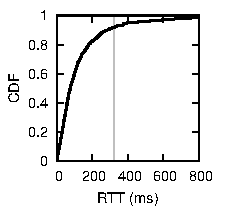
\includegraphics[width=0.3\textwidth]{figures/Via-Quality-CDF-RTT.pdf}
        \label{subfig:}
}
\subfloat[\small{Loss}]
{
        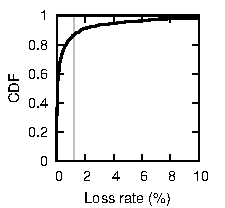
\includegraphics[width=0.3\textwidth]{figures/Via-Quality-CDF-Loss.pdf}
        \label{subfig:}
}
\subfloat[\small{Jitter}]
{
        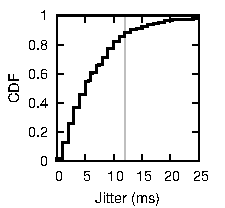
\includegraphics[width=0.3\textwidth]{figures/Via-Quality-CDF-Jitter.pdf}
        \label{subfig:}
}
\caption{CDF of observed network performance metrics -- 
RTT, loss rate, jitter. Vertical grey lines show the thresholds 
for poor network performance.}
\label{fig:perf-cdf}
\end{figure}

\mypara{Thresholds of network performance} 
Figure~\ref{fig:perf-cdf} shows the distribution of network 
performance experienced by calls   using default routes. 
A significant fraction of calls (over $15\%$) occur on paths with 
RTT over $320$ms, or loss over $1.2\%$, or jitter more than 
$12$ms, which we pick as our {\em thresholds for 
poor performance}. % These values correspond to a PCR of $0.3$ (Figure~\ref{fig:pcr}). 
These values are in line with literature from industry 
and standards bodies that recommend one-way end-to-end 
delay of no more than $150$ ms and a packet loss rate of 
no more than $1\%$ for good call quality~\cite{cisco-voip, itu}. 
%Also, these thresholds match with the average values of RTT, loss and jitter of the user-defined ``poor'' calls.\vnp{I believe Ross had expressed the concern that the previous sentence might be leaking information. I think we can just strike it out.} 
Note that these thresholds are on the {\em average} 
values over the call's duration during which there may 
be transient spikes (e.g., loss burst) in bad performance.

% justified shortly ahead. %% VS: UNCLEAR  WHAT NEEDS TO BE JUSTIFIED?
 
%Finally, with these thresholds, the MOS score with the equation above works out to 3.5, which lies between "fair" (3) and "good" (4)~\cite{itu-mos}. However, as indicated above, the distribution of user experience corresponding to a mean score of 3.5 could, nevertheless, span a "poor" user experience on some calls. 

%Therefore, we pick $320$ms, $1.2\%$, and $12$ms, respectively, as the thresholds for RTT, packet loss rate, and jitter. We note that the literature from industry and standards bodies  also indicates requirements such as a one-way end-to-end delay of no more than 150 ms and a packet loss rate of no more than 1\%~\cite{XXX http://www.cisco.com/c/en/us/td/docs/ios/solutions_docs/qos_solutions/QoSVoIP/QoSVoIP.pdf, https://www.itu.int/rec/T-REC-G.114/en XXX}, which are in line with these thresholds.
	 
\mypara{Our focus: Poor Network Rate}
We define the {\em poor network rate} (PNR) of a network 
metric for a set of calls as the fraction of calls whose performance 
on the metric is worse than the chosen thresholds: 
RTT $\geq 320$ms, loss rate $\geq 1.2\%$, jitter $\geq 12$ms. 
One of our goals is to reduce PNR of {\em each} individual metric 
 (i.e., how often each of them is poor). 

However, as there could be dependencies between network 
metrics, improving one metric may increase PNR of another 
metric. 
Figure~\ref{fig:perf-correlation} shows the three pair-wise 
correlations. 
While the plot is based on an aggregation of data across all 
calls and paths, the substantial spread suggests at least the 
possibility that improving one performance metric {\em could} 
lead to a worsening of the other metrics. 
Therefore, we also focus on reducing PNR of three metrics 
collectively, i.e., minimizing how often {\em at least one} of 
the metrics is poor.

{\em How well does PNR on average values compare to 
using full packet traces?} 
Analysis of a subset of ($70$K) calls with full packet traces 
shows that $80\%$ of calls rated ``non-poor'' using the 
thresholds on average metrics (``at least one poor metric'') 
have a (packet-trace based) MOS score higher than 
three-quarters ($75\%$) of calls rated ``poor'' using the 
average metrics. We run a proprietary MOS calculator 
on the packet traces that contain send/receive timestamps 
for each packet and loss information. 
This shows that defining the thresholds on average values 
of the call is a reasonable approximation.


%Our goal is to reduce the PNR, so we focus on 
%the calls for which the network metrics exceed their respective thresholds and look to improve their performance.% via intelligent relay selection in the context of a managed overlay network.}

% via managed relays and quantify the potential improvement in \xref{sec:potential}. %Sure large RTTs could arise because call may be relayed for reasons of connectivity (e.g., firewall or NAT traversal) rather than performance improvement.

%\myparatight{Are network metrics correlated?} 
%We expect that improving performance of one metric would, on average, result in an improvement in the other metrics too. Figure~\ref{fig:perf-correlation} shows two examples of pair-wise correlations. Such correlations have a direct bearing on the desirability or otherwise of a relayed path.
%% are overall helpful when deciding on relays. However, 
%%The substantial spread, as indicated by the overlapping box plots, indicates that a better value of one metric may not necessarily correspond to a better value of the other metrics. 
%While the plot is based on an aggregation of data across all calls and paths, the substantial spread suggests at least the possibility that even for an individual call, improving one performance metric {\em could} lead to a worsening of the other metrics. Therefore, we focus on reduction in PNR both on the individual metrics as well as collectively.
%Therefore, when a relaying decision is made, it is important to pay careful attention to each of the network metrics. 
%%%\red{The Jacquard coefficients shown in XXX quantify the extent of co-occurence of poor performance across the three network metrics. We note that XXX}

%\vnp{It is unclear implies for an individual call. Sure, across all calls and paths, one with a smaller RTT could, in fact, have a higher loss rate than another with a larger RTT. However, it doesn't really mean that such reversal would happen if one metrics were optimize for an individual call}

\begin{figure}[t!]
\centering
\subfloat[\small{RTT vs. loss rate}]
{
        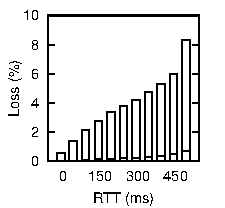
\includegraphics[width=0.3\textwidth]{figures/Via-Quality-Correlation-RTT-loss.pdf}
        \label{subfig:}
}
\subfloat[\small{RTT vs. jitter}]
{
        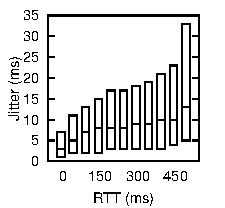
\includegraphics[width=0.3\textwidth]{figures/Via-Quality-Correlation-RTT-jitter.pdf}
        \label{subfig:}
}
\subfloat[\small{Jitter vs. loss rate}]
{
        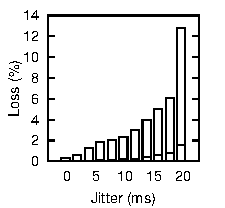
\includegraphics[width=0.3\textwidth]{figures/Via-Quality-Correlation-jitter-loss.pdf}
        \label{subfig:}
}
\caption{Pair-wise correlation between performance metrics. 
The Y-axis shows the distribution ($10^{\text{th}}$, $50^{\text{th}}$, 
$90^{\text{th}}$ percentiles) of one metric as a function the other 
metric over the same set of calls.}
%\ga{Only 25th, median, 90th? Also jitter vs. loss}
\label{fig:perf-correlation}
\end{figure}













\subsection{Spatial Patterns}
\label{subsec:measurement:voip:spatial}

We have seen in 
Section~\ref{subsec:measurement:voip:quality} that user 
experience is sensitive to poor network performance 
and that a significant fraction of calls suffer from poor 
performance when using \direct routing. 
Next, we analyze whether the calls with poor networks 
share common patterns. This subsection focuses on 
{\em spatial} patterns while
Section~\ref{subsec:measurement:voip:temporal} 
looks at {\em temporal} patterns.

% We define the {\em poor network rate} (PNR) for a given set of calls as the fraction of calls whose network performance is worse than the thresholds: RTT $\geq 320$ms, loss rate $\geq 1.2\%$, jitter $\geq 12$ms. PNR can be measured both on the individual metrics (how often were each of them poor?) as well as collectively (how often was {\em at least one} of the metrics poor?). Recall from Figure~\ref{fig:perf-cdf} that these thresholds correspond to the user-specified poor call rate (PCR) of $0.3$.
% to poor call performance with a probability of $0.5$. 

\begin{figure}[t!]
\centering
\subfloat[\small{International vs. domestic}]
{
        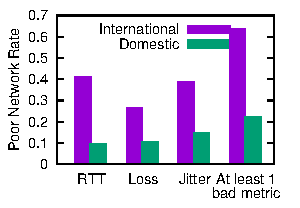
\includegraphics[width=0.45\textwidth]{figures/Via-Opportunity-International.pdf}
        \label{subfig:opportunity-international}
}
\subfloat[\small{Countries of one side of a call}]
{
        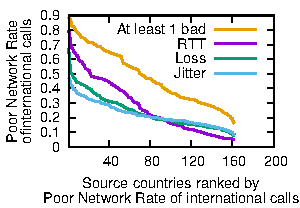
\includegraphics[width=0.45\textwidth]{figures/Via-Opportunity-International-ByCountry.pdf}
        \label{subfig:international-bycountry}
}
\caption{International vs. Domestic Calls.}
\label{fig:country}
\end{figure}

\mypara{International vs. Domestic calls} 
On all three network metrics, we see that international 
calls (between users in different countries) have a
 higher PNR, i.e., they are more likely to suffer from 
 bad network performance than domestic calls. 
Figure~\ref{fig:country} shows a $2-3\times$ higher 
PNR on international calls than on domestic calls. 
The figures also show the fraction of calls with at least 
one metric being poor (the last pair of bars), where the 
gap between international and domestic calls is even 
larger. 
Though conclusively diagnosing the root cause of bad 
performance on international calls is hard and beyond 
the scope of this work, the higher PNR for international 
calls points to the WAN path as the culprit.\footnote{One 
aspect is that users tend to use VoIP 
regardless of its performance for international calls, 
unlike domestic calls.} %\cmrvnp{we speculate that it is because ISPs have less incentive to ensure good quality for international calls than domestic ones.}}

% \vnp{The "at least 1 bad metric" bars seem at least as tall as the other bars stacked up, which suggests that there is little overlap between the subsets for which each metric is poor.}

To understand this further, 
Figure~\ref{subfig:international-bycountry} zooms into 
the international calls and classifies them by the country 
of the callers (source). 
We see that there is a skewed distribution, with certain 
countries having a PNR as high as on the individual metrics. 
The PNR of international calls across the remaining 
countries drops gradually but half of them still see a 
non-negligible PNR of $25\%-50\%$. 
This suggests that poor network performance is 
quite widespread, highlighting the suitability of a 
{\em globally} deployed overlay network that provides 
high performance inter-connection between overlay nodes.
% and calling for a selective approach to routing via the managed network. 
% but the overall distribution is flat, indicating that most countries do not have particularly poor network performance. 

%\begin{figure}[t!]
%\centering
%\hspace{-0.5cm}
%\subfigure[Inter-domain vs. intra-domain]
%{
%        \includegraphics[width=0.25\textwidth]{new-figs/Opportunity-Interdomain.pdf}
%        \label{subfig:opportunity-interdomain}
%}\hspace{-0.5cm}
%\subfigure[Source AS]
%{
%        \includegraphics[width=0.25\textwidth]{new-figs/Opportunity-Interdomain-ByAs.pdf}
%        \label{subfig:interdomain-byas}
%}\hspace{-0.5cm}
%\ncaption{Inter-domain vs. Intra-domain Calls.}
%\label{fig:domain}
%\end{figure}

\mypara{Inter-AS vs. Intra-AS Calls} % The above trends persist when we splice calls by the AS domains of the source and destinations. 
Similar to international calls, calls across ASes 
are $2-3\times$ more likely to experience poor 
network performance than those within the same 
AS domain. %Also, while calls originating from a small fraction of the ASes have a much higher PNR, the overall distribution is even. 
%This, again, points to the need for a selective approach to routing via the global managed overlay.
This, again, points to the need for enabling alternatives to default routing to improve WAN performance.
% a relay system that provides wide-area routing of better performance.

\begin{figure}[t!]
\centering
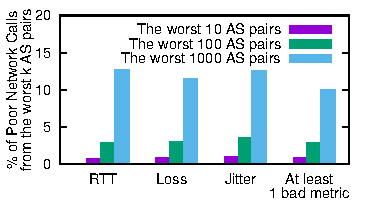
\includegraphics[width=0.6\textwidth]{figures/Via-BadContribution-Top-AsPair.pdf}
\caption{The percentage of calls over poor network 
conditions that come from the worst $n$ AS pairs; 
AS-pairs are ranked in descending order of their 
contribution to total amount of calls with poor performance.}
 %\ga{Change ``top'' to ``worst''.}
\label{fig:bad-contribution}
\end{figure}

\mypara{Not just a few problematic source-destination pairs}
Contrary to our expectation, a few source-destination pairs 
alone do {\em not} account for a big chunk of the PNR. % Our hypothesis was to observe the commonly occurring ``Pareto'' effect.
 Figure~\ref{fig:bad-contribution} shows the fraction of 
 calls that suffer from poor network performance from the 
 worst AS pairs, ranked in order of their contribution to the 
 overall PNR. %Across different metrics, we see that the calls with poor network metrics are not limited to a handful of AS pairs. 
Even the worst $1000$ AS pairs together only count for less 
than $15\%$ of the overall PNR. %\vnp{I'm unable to reconcile these numbers with the bars depicted in Fig 5.} 
This means that localized solutions that fix a few bad ASes 
or AS pairs, e.g., informing the AS administrators or the 
clients directly regarding their ISPs, are not sufficient. 
 
%\vnp{Absolute counts don't quite tell the full story. We should also report what fraction of all AS pairs seen is represented by k}
 
While the above analysis was at the granularity of ASes, 
we also tested at other, finer granularities (e.g., $/24$ and 
$/20$ prefixes of the caller and callee IP addresses) and 
found similar results (of not just a few culprits).
In fact, for the pairs with sufficient data density at the $/24$ 
granularity, we found that performance distributions of the 
network metrics were similar to those at the granularity of ASes.% are close to those at the granularity of $/24$; for instance, on more than 85\% $/24$ pairs where we have at least 10 calls, the average RTT is within 50\% away from that of the corresponding AS pairs.



\begin{figure}[t!]
\centering
%\subfigure[Timeseries\jc{Needs to be changed}]
%{
%        \includegraphics[width=0.45\textwidth]{new-figs/Timeseries-badrate.pdf}
%        \label{subfig:temporal-structure-timeseries}
%}
\subfloat[\small{Persistence}]
{
        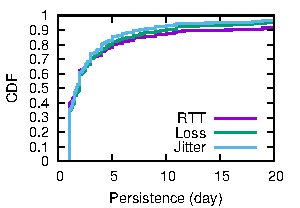
\includegraphics[width=0.45\textwidth]{figures/Via-Persistence-AsPair.pdf}
        \label{subfig:temporal-structure-persistence}
}
\subfloat[\small{Prevalence}]
{
        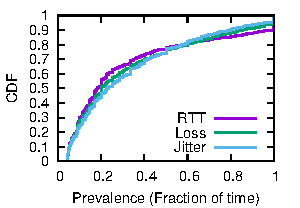
\includegraphics[width=0.45\textwidth]{figures/Via-Prevalence-AsPair.pdf}
        \label{subfig:temporal-structure-prevalence}
}
\caption{Temporal patterns of poor network performance. 
Figure~\ref{subfig:temporal-structure-persistence} and 
\ref{subfig:temporal-structure-prevalence} show the distribution of 
the persistence and prevalence of AS pairs having high PNR.}
\label{fig:temporal-structure}
\end{figure}









\subsection{Temporal Patterns}
\label{subsec:measurement:voip:temporal}

We now analyze temporal patterns of poor network 
performance. 
We perform this analysis by grouping the 
performance of AS pairs into $24$-hour time 
windows.\footnote{Different grouping granularities
yielded similar observations.}
We conservatively label an AS pair as having 
{\em high PNR} for a specific metric (on a given day) if 
its PNR on that day is at least $50\%$ higher than the 
overall PNR of all calls on that day. 

%Knowing what types of calls are more likely to have poor performance, however, does not mean they can be easily fixed. Next, we study the spatial and temporal patterns of bad network performance, and show that fixing a handful of AS pairs in specific time periods does not address most of them, which suggests the needs for a system that can adaptively alleviate bad network performance for users all over the world.

%\myparatight{Methodology} To understand the spatial and temporal patterns of bad network performance, we consider the performance distribution of each AS pair within different time windows of 24 hours. We first group the calls based on the pair of source and destination AS, and to ensure statisical significance, we consider each AS pair that have at least 20 calls in each day\footnote{We decide to group calls by source and destination AS pair on a daily base because it is the finest granularity that still have enough calls for most of the time. We used different grouping granularities and found qualitatively similar observations.}. 
%\ga{Let's see if we can argue for AS-level analysis as reasonable. Maybe present some /24 granularity data, show that the trends are similar when there is sufficient data, and say we will use AS-level data owing to the density? As we have all discussed before, it is not a natural granularity to pick unless we say why so.}

Figure~\ref{subfig:temporal-structure-persistence} and 
\ref{subfig:temporal-structure-prevalence} show the 
distribution of {\em persistence} and {\em prevalence} of 
high PNR AS-pairs. 
The {\em persistence} of an AS pair is the median 
number of consecutive days when it has high PNR. 
The {\em prevalence} of an AS pair is the fraction of 
time it has high PNR.
The figures show a highly skewed distribution with 
$10\%-20\%$ AS pairs always having high PNR, while 
$60\%-70\%$ AS pairs have poor performance for less 
than $30\%$ of time and lasting no longer than one 
day at a stretch. 
%These majority of AS pairs whose poor network performance is neither prevalent nor persistent should be improved in a dynamic manner.
%This means the poor performance of most AS pairs is neither prevalent nor persistent.
%This means that to fix the majority of AS pairs that are neither prevalent nor persistent that statically configuring a solution to improve only the (relatively few) most prevalent and persistent AS pairs is not sufficient; 
This observation suggests that instead of statically 
configuring the system to improve performance for 
only the (relatively few) most prevalent and persistent 
AS pairs, we need to dynamically decide if a call 
should use default Internet routing or be relayed. % sent through overlays.
%It reinforces the point 
%, in order to improve performance for the majority of AS pairs. 





\subsection{Key Observations}
\label{subsec:measurement:voip:findings}

The key observations from this section are:
\begin{enumerate}
\item {\em Network performance matters.} User experience of 
calls is impacted by even small changes in network metrics. 
\item {\em Wide-area} communication, such as international 
and inter-domain calls, are more prone to bad network performance, 
and have a large room of improvement.
\item Calls suffering from poor networks are spread {\em spatially} 
(across ASes) and {\em temporally}. %Most calls with poor network performance are not from a handful of source-destination AS pairs. And most source-destination pairs only experience high PNR for a relatively short period of time.
\end{enumerate}

%These observations motivate the need for a network overlay (Observation 1) that provides better paths with a {\em global} footprint of overlay nodes (Observation 2), and the need to choose routes {\em selectively} and {\em dynamically} (Observation 3). 
